%!TEX root = thesis_main.tex

\chapter{Design and Analysis of a two stage Cycloid}\label{ch:dual}
% Give the abstract for a 2-stage 
% People did not put many numbers on pages for these things 
% We built one based on the available information, that lead us to understand many of the deficiencies and to further investigate, leading to the equations I'm presenting before you. 

In recent literature, authors have proposed new concepts for cycloidal drives. A notable addition to the recent literature is a ``two-stage'' design that multiplies the cycloid reduction substantially in a very small package \cite{ref:new_two_stage}. Traditionally, a two-stage reduction takes the output of the first stage and sends it in as the input of the second stage in a stand-alone reduction. However, in the newly proposed ``two-stage'' cycloid, the first stage is directly coupled to the second, generating a potentially very large ratio in a small package. This concept is very intriguing for systems that need very large reductions and have space limitations. 

With the recent advent of this style of design, there still exists many unexplored elements of the design of this drive. The kinematic layout and profile generating equations have been developed, as well as the precautions necessary for machining tolerances, as well as an initial development of the force calculations for one design. These are discussed in Section \ref{ch:dual:initial_equations}. Using the available literature, our group at NASA: Johnson Space Center developed a two-stage cycloid with a fused and counterbalanced set of cycloid plates, discussed further in Section \ref{TODO}. Through these tests, gaps in the analysis of the motion and forces present in the new two-stage concept were identified, specifically pertaining to the loads and relative motion necessary in the interaction between the lobes and housing, and the subsequent losses they generate. This gap is closed in the analysis of this thesis, covered in Section \ref{ch:dual:equations}

\todo[inline]{may need to add a chapter or section about more explicit design of ours? or de-emphasize in the above paragraph}

Through this analysis, the new two-stage cycloid is demonstrated to have potentially large efficiency losses inherent to its design. If the cycloid is designed in a similar fashion to a compact single-stage design with pins that can float in the housing, the generated forces and sliding that exists in the single-stage is multiplied in this design, resulting in low peak efficiencies considering just the lobe to pin interaction, 40\% for the example design with a coefficient of friction of 0.1. This analysis is presented in Section \ref{ch:dual:test_results} and shows that for a new two-stage cycloid to run effectively, rolling elements may need to be introduced between for the housing rollers, with a more in depth discussion in Section \ref{ch:dual:discussion}.

\todo[inline]{somewhere I should talk about the neat new ways that people are proposing to minimize the losses, maybe this goes in 2 instead}.

\section{Two-Stage Cycloid Design} \label{ch:dual:initial_equations}
% Go over the 4 papers and talk about what they say, how it's derived, and finish with "what they're missing" 
% - present the way math behind my derived values, changes of frame etc. 

The traditional approach to a mutli-stage gearbox is to take the output of the first stage, and use it as the input to a second reduction. Blagojevic et. al. proposed a new concept for the design of a two-stage cycloid reduction in 2011 in which, a the first cycloid plate is connected through pins to a second cycloid plate with a different number of lobes. These lobes interact with a second set of pins that are allowed to rotate, and induces a large reduction through into the housing pins of this ``second stage.'' \cite{ref:new_two_stage}. This section will first detail the motion of the system, and then present the generating equations to lay the foundation for the continued analysis. 

\subsection{New Two-Stage Conceptual Design} \label{ch:dual:initial_equation:motion}

The designs presented in the initial work by Blagojevic et. al., as well as the additionally proposed design concepts by Lin et. al. \cite{ref:two_stage_tooth_mod} and Hseih and Jian \cite{ref:hsieh_effect_2016} are predicated on the transfer of the eccentric wobble and counter-rotation of a traditional single cycloid plate to a second cycloid plate with a different number of lobes and rollers. The second set of rollers is mounted to a bearing as the output of the system. It is the transfer of this motion from the first plate to the second plate that generates the motion to the second set of housing pins. A simple cross section of a traditional two-stage cycloid versus the new concept can be seen in Fig. \ref{fig:two_stage_simple_cross}. 

\begin{figure}[h]
	\centering
	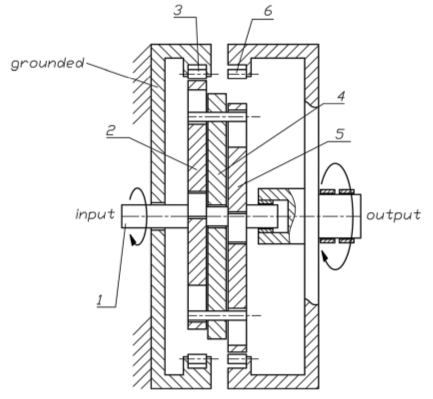
\includegraphics[width=0.48\linewidth]{fig/new_layout_TODO}
   \caption{TODO: The newly proposed layout for a two-stage cycloid
   \\ Figure adapted from Blagojevic et. al. \cite{ref:new_two_stage}}
   \label{fig:two_stage_simple_cross}
\end{figure}

The proposed designs in the literature transform the first stage plates counter-rotation to the second stage plate via output rollers similar to those found in a single-stage design. These rollers are rigidly connected to the second stage plate, which sits 180\textdegree offset eccentricity of the first stage plate to counterbalance the vibrations in the actuator \cite{ref:new_two_stage}, these elements are noted in Fig. \ref{fig:two_stage_simple_cross}. The design was further elaborated with a rigid plate connecting the pins that transfer load from the first cycloid plate to the second, allowing increased rigidity. 

The NASA design proposes a new layout option that decreases the number of rolling elements by fusing the two cycloid plates and allowing them to rotate together rather than 180\textdegree out of phase. This eliminates the rolling element of the pins between the first and second cycloid plate. However, this also eliminates the natural vibration elimination, so a counterbalance must be added to the input shaft. In the design of the actuator, this weight trade between the two designs was negligible, and an efficiency increase should be achieved. The assembly for this design style can be seen in Fig \ref{fig:two_stage_design} 

\begin{figure}[h]
	\centering
	\includegraphics[width=0.50\linewidth]{fig/two_stage_motion}
   \caption{TODO Create a drawing of the two-stage we designed, either in real CAD or similar to the simple cross section graphic}
   \label{fig:two_stage_design}
\end{figure}


\subsection{New Two-Stage Profile Generation} \label{ch:dual:initial_equation:profiles}
% Go through equations that generate the profile, introduce alpha. 

To begin a design, the first thing a designer needs is the reduction of the system. This is given plainly by Lin et al. and is reproduced in equation \ref{eq:two_stage_ratio_again}.

\begin{equation} \label{eq:two_stage_ratio_again}
Q = \frac{1}{1 - \frac{N_1 (N_2-1)}{N_2 (N_1-1)}}
\end{equation}

There are two interesting items to note in this reduction equation. First, the resulting ratio is not the traditional single-stage ratio of the first cycloid plate lobes and pins multiplied by the single-stage ratio for the second cycloid plate and pins. This is only the case when the lobes are different by just one pin. Therefore, a large gambit of ratios can be created using this style, and due to the load sharing across all of the lobes of both stages, large torque carrying capacities are possible. Second, the ratio can be positive or negative, meaning the output can spin in the same direction as the input (positive ratio) or the opposite direction (negative ratio). Due to the symmetry of the loads required, this has a very minor practical impact to the load distribution, but does result in changes in the efficiency of the system and will be further discussed in Section \ref{ch:dual:equations}. 

\begin{figure}[h]
	\centering
	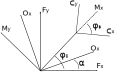
\includegraphics[width=0.50\linewidth]{fig/two_stage_frames}
   \caption{Coordinate frames used for calculating the profiles for the first and second stage cycloid plates, as well as the resultant angles from the induced motion \textalpha.}
   \label{fig:two_stage_frame}
\end{figure}

The second step in the design process is the generation of the cycloid plate profiles. These profile equations are adapted directly from the single-stage design equations in Section \ref{ch:design:basic_calc:profile}. An addition can be made for the generating equations for the second stage design that account for the motion of the output pins that will be useful for later calculations. In Figure \ref{fig:two_stage_frame}, an additional frame is added, the output frame \textit{O} relative to the fixed frame. This is the frame that the output pin rotates in with a transformation matrix 

\begin{equation} \label{eq:T_fo}
T_f^o = \left[{\begin{array}{cccc}
		cos(\alpha) & -sin(\alpha) & 0 & 0\\
		sin(\alpha) & cos(\alpha) & 0 & 0\\
		0 & 0 & 1 & 0\\
		0 & 0 & 0 & 1 \end{array} } \right]
\end{equation}
The second stage can be generated with any desired offset from the first stage, it will only change the initial meshing of the output, but will have no impact on the functionality of the design. 

Using this new design concept and the basic definitions of the lobe profiles, the profiles for the two-stage design can be simply created. For the example design, the actuator was designed with the following parameters. 
\begin{table}[h]
  \vskip0.2cm
  \caption{Design parameters for manufactured fused two-stage design}
  \label{table:two_stage_design_params}
  \begin{center}
    \vskip-0.2cm
	\begin{tabular}{|c|c|c|}
		\hline
		Variable & Symbol & Value\\
		\hline
		Stage 1 Housing Rollers & \textit{N\textsubscript{1}} & 19\\
		\hline
		Stage 1 Lobes & N/A & 18\\
		\hline
		Stage 2 Housing Rollers & \textit{N\textsubscript{2}} & 18\\
		\hline
		Stage 2 Lobes & N/A & 17\\
		\hline
		Total Ratio & Q & 324:1 \\
		\hline
	\end{tabular}
  \end{center}
\end{table}
\todo[inline]{add the other values like diameter and roller size}

Through the analysis, this will be contrasted with a design that inverts the ratio via the given parameters. 

\begin{table}[h]
  \vskip0.2cm
  \caption{Design parameters for an inverted ratio to the manufactured fused two-stage design}
  \label{table:two_stage_invert_design_params}
  \begin{center}
    \vskip-0.2cm
	\begin{tabular}{|c|c|c|}
		\hline
		Variable & Symbol & Value\\
		\hline
		Stage 1 Housing Rollers & \textit{N\textsubscript{1}} & 18\\
		\hline
		Stage 1 Lobes & N/A & 17\\
		\hline
		Stage 2 Housing Rollers & \textit{N\textsubscript{2}} & 19\\
		\hline
		Stage 2 Lobes & N/A & 18\\
		\hline
		Total Ratio & Q & -323:1 \\
		\hline
	\end{tabular}
  \end{center}
\end{table}



\section{Development of Two-Stage Design Equations} \label{ch:dual:equations}
% Go over what I have invented
% - the motion equations of the pins 
% - The load equations on the pins 
% - the projected efficiency of the system. 

After the basis of the design for the two-stage system has been laid out, more calculations are necessary for proper design of the system. First, the force equations on the lobes will be laid out fully to allow for load calculations on the lobes and pins. Then, using the basis for the relative sliding velocity laid out in Section \ref{ch:design:pin_roll_1s:sliding_equations}, the relative sliding at each point will be determined. This will provide a basic estimate of loss for a two-stage cycloid system due to the interactions between the lobes and rollers. 

\subsection{Two-Stage Lobe Force Calculations} \label{ch:dual:equtions:force}

The force equations for the interaction between the lobes and rollers on the new two-stage system is initially laid out by Blagojevic et al. \cite{ref:new_two_stage}. However, this is for the decoupled cycloid plates. Therefore, a new set of equations is necessary for the calculation of the forces on the fused cycloid plate design. The initial equations for the derivation are presented in Section \ref{ch:design:single:force_analysis} and are based off of the work by Malhorta and Parameswaran \cite{ref:malhorta_2}. 

If a simple set of figures are made to show the force balance for the fused two-stage design, some interesting observations can be made. Figure \ref{fig:two_stage_force_pos} shows the forces resisting a the positive rotation of a positive ratio, the figure \ref{fig:two_stage_force_neg} shows the forces for a negative ratio. In these two figures, it is clear that the sides the forces are acting on must flip in order to maintain the force balance. While this is an intuitive result, it's physical implications for design are important. In a typical cycloid, the forces occur only on the sector that the motor's eccentric arm is on, so it is moving with the eccentricity. Generally, cycloids are designed with machining tolerances to prevent excessive contact on the non-force sides, so contact only occurs on the eccentric side of motion. However, in the fused plate design, there is force being transmitted opposite of the eccentricity. Therefore, when designing in this manner, great care must be taken to ensure close meshing of the cycloid plates on all sides to limit the losses in material deflection that would otherwise need to occur to carry the load. 


\begin{figure}[h]
	\centering
	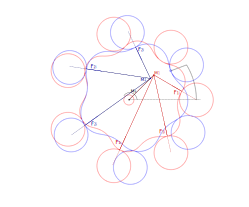
\includegraphics[width=0.80\linewidth]{fig/two_stage_loads_pos}
   \caption{The forces acting on a fused two-stage cycloid. The loads on the first stage in this arrangement, shown in red, are in the opposite direction of a typical single-stage cycloid and act through the instant center, M1 and act on the trailing edge with respect to the eccentricity while the loads on the second stage, shown in blue, are in a more typical arrangement to a single stage and pass through the point M2. }
\end{figure}

\begin{figure}[h]
	\centering
	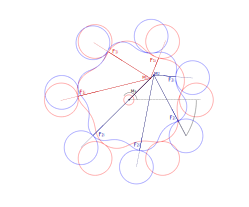
\includegraphics[width=0.80\linewidth]{fig/two_stage_loads_neg}
   \caption{The forces acting on a fused two-stage cycloid. The loads on the first stage in this arrangement, shown in red, are identical to that found in a single-stage, passing through the instant center M1. The reaction forces on the second stages, shown in blue, act on the opposite side of the eccentricity through point M2. }
   \label{fig:two_stage_force_neg}
\end{figure}

The next important observation from these force diagrams is that the force is acting on a different line for the first stage and the second stage plates. These forces act in line with the instant center that was used to generate the profile, but as noted previously, the instant center used to generate the second stage profile is different than the instant center that is actually induced by the motion of the first stage. This phenomena will be critical to do the development of the relative motion equations in Section \ref{ch:dual:equations:vel} and the force equations in this section. 

The force calculations for the two-stage fused cycloid plate are very similar to those laid out in Section \ref{ch:design:single:force_analysis}, but instead of the balancing output forces acting on the output pins, they act on the lobes of the second stage. The forces on the first stage are denoted as \textit{F\textsubscript{1i}} and the forces on the second stage are denoted \textit{F\textsubscript{2j}}, with an input force \textit{F}. The dimensions used for calculation for the first stage are identical to those used in a single-stage design (equation [\ref{eq:single_b} - \ref{eq:single_l}). There are only two modifications necessary to calculate these parameters for the second stage. First \textit{N\textsubscript{1}} is substituted for \textit{N\textsubscript{2}} and \textrho\ is calculated using the new \textit{N\textsubscript{2}}. Second, a slight modification must be made to \textbeta, and can be seen in Fig \ref{fig:two_stage_force_beta}. \textbeta\ must be adjusted by the output angle \textalpha resulting in the physical parameters for calculating the second stage of 


\begin{equation} \label{eq:single_b_2}
\beta_{2j} = \frac{2\pi j}{N_2} + \gamma
\end{equation}
\begin{equation} \label{eq:single_d:x_2}
d_{2x} = R \cos(\beta_j) - E N_2 \cos(\phi_2)
\end{equation}
\begin{equation} \label{eq:single_d:y_2}
d_{2y} = R\sin(\beta_j) - E N_2 \sin(\phi_2)
\end{equation}
\begin{equation} \label{eq:single_d_2}
d_2 = \sqrt{d_{2x}^2 + d_{2y}^2}
\end{equation}
\begin{equation} \label{eq:single_gamma_2}
\gamma_{2j} = \sin^{-1}\left[{\frac{R \sin{\beta_j - \phi_2}}{d_2}}\right]
\end{equation}
\begin{equation} \label{eq:single_rho2_2}
\rho_{22} = \rho_{21} - E
\end{equation}
\begin{equation} \label{eq:single_l_2}
l_{2j} = \rho_{22} \sin{\gamma_{2j}
\end{equation}

\begin{figure}[h]
	\centering
	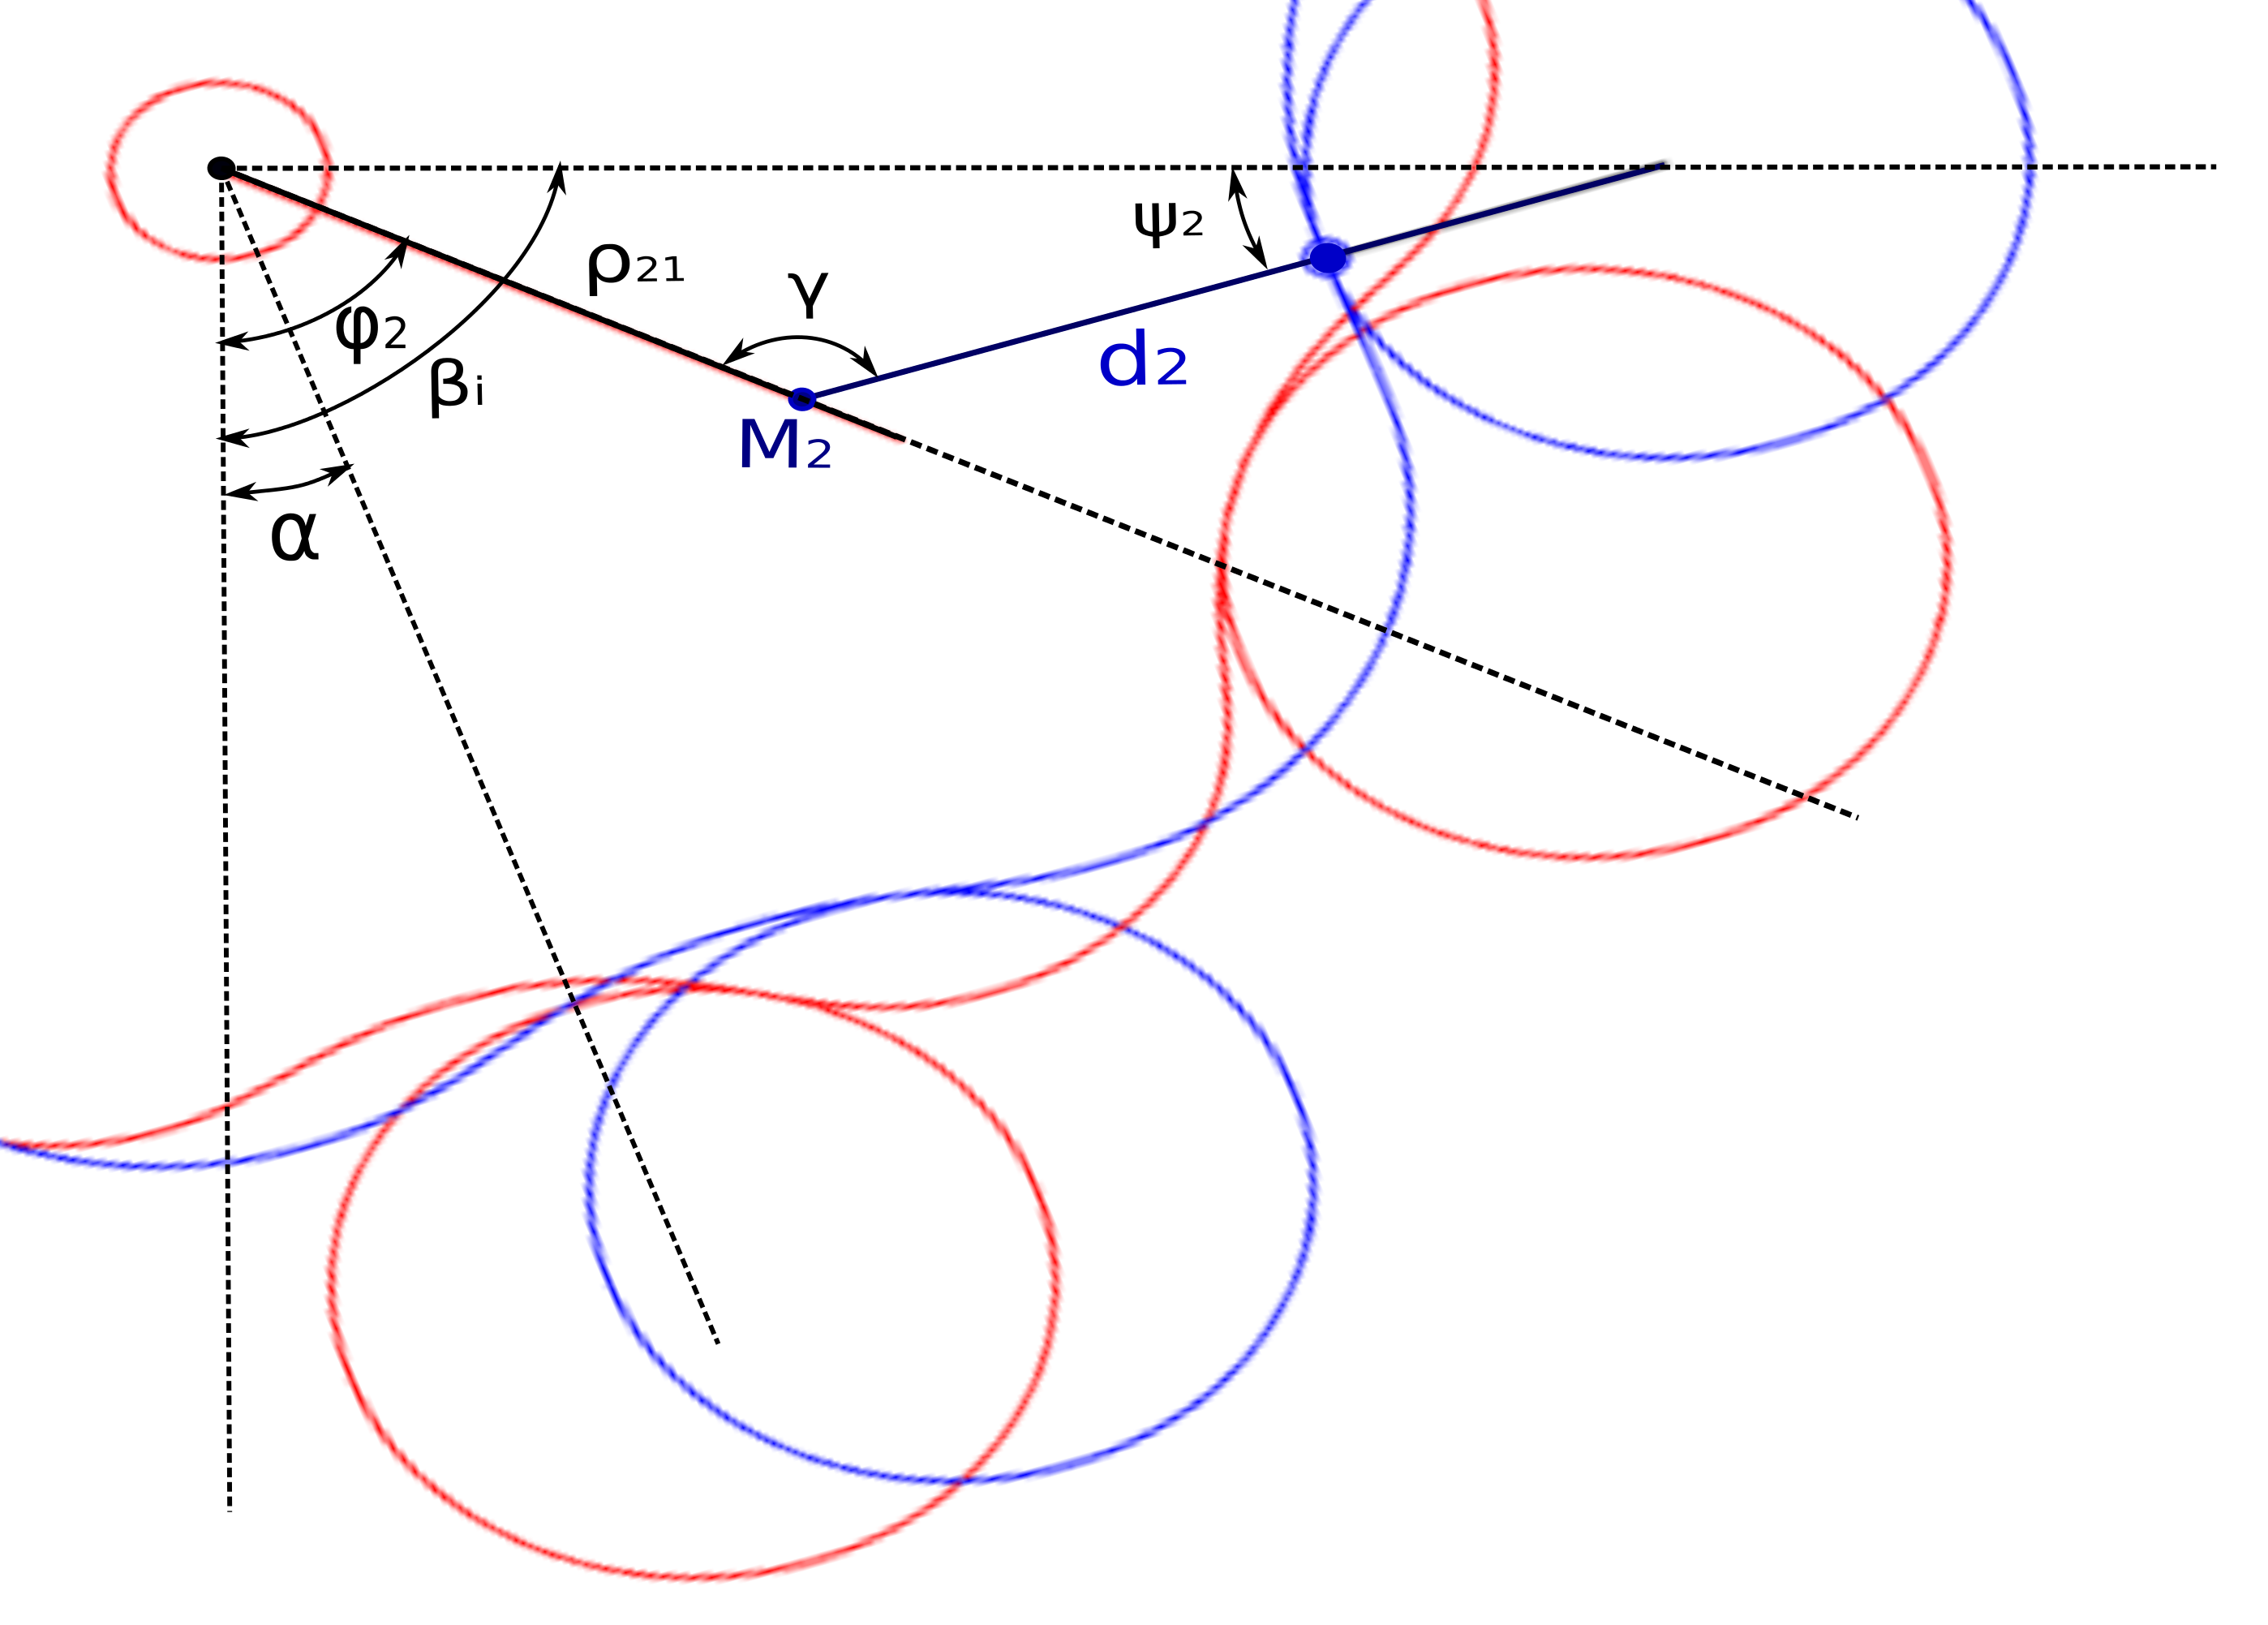
\includegraphics[width=0.8\linewidth]{fig/two_stage_loads_angles_2}
   \caption{Angles necessary for calculting the forces on the second stage of the cycloid-plate. The calculations are nearly the same as a single-stage save a necessary modification to \textbeta\ due to the movement of \textalpha.}
   \label{fig:two_stage_force_beta}
\end{figure}

Using these design parameters and the knowledge that the number of pins in contact on the first stage, \textit{N\textsubscript{1c}} and second stage, \textit{N\textsubscript{2c}} are half or fewer than the total number of pins

\begin{equation}
N_{1c} = \frac{N_{1} - 1}{2},\ if\ (N_1 -1)\ is\ even 
\end{equation}
\begin{equation}
= \frac{(N_{1}-1) - 1}{2},\ if\ (N_{1} - 1)\ is\ odd 
\end{equation}
\begin{equation}
N_{2c} = \frac{N_{2}-1}{2},\ if\ (N_{2}-1)\ is\ even 
\end{equation}
\begin{equation}
= \frac{(N_{2}-1) - 1}{2},\ if\ (N_{2}-1)\ is\ odd 
\end{equation}

the force equations become 

\begin{equation} \label{eq:dual_power}
M_a = \frac{R}{Q} \sum_{j=1}^{N_{2c}} F_{2j} l_{2j}
\end{equation}
\todo[inline]{look into this equation more}
\begin{equation} \label{eq:dual_input}
Ma = F E \cos(N_1 \phi_2 + \gamma)
\end{equation}
\begin{equation} \label{eq:dual_torqe}
\sum_{i=1}^{N_{1c}}F_{1i} l_{1i} - \sum_{j=1}^{N_{2c}}F_{2j} l_{2j} = 0
\end{equation}

\begin{equation} 
\frac{F_{1i}}{l_{1i}} = constant 
\end{equation}
\begin{equation}
\frac{F_{2j}}{l_{2j}} = constant
\end{equation}

Using these equations, the forces on each of the lobes and pins can be obtained. THe results of this analysis will be presented in Section \ref{ch:dual:test_results}.

\subsection{Lobe to Pin Contact Velocity for Two-Stage Designs}\label{ch:dual:equations:vel}
% THIS FITS INTO THE NEXT SECTION, THE QUESTION IS WHERE...
To begin to understand the losses present in the two-stage cycloid system, the sliding interactions are necessary to derive between all of the pins and rollers, similar to those set out in Section \ref{ch:design:pin_roll_1s:sliding_equations}.

An important distinguish can be made between a single-stage cycloid and the two-stage concept using Figure \ref{fig:second_stage_angle}. The profile for a cycloid is generated based off of Kennedy's Theorem, discussed in Section \ref{ch:design:basic_calc:profile} which places the contact point along the straight line from the center of the housing pin to the line of centers of the motor and the cycloid plate. This distance is defined as 
\begin{equation}
D_2 = N_2 E
\end{equation} 
where \textit{N\textsubscript{2}} is the number of housing rollers in the second stage. However, because the first and second stage plates are fused, the actual instant center of the plate must be the instant center dictated by the first stage motion at 
\begin{equation}
D_1 = N_1 E 
\end{equation} 
defined by the number of rollers \textit{N\textsubscript{1}} in the first stage. Therefore, the same simplification that was used in the single-stage cannot be applied to both stages in the two-stage concept. 

\begin{figure}[h]
	\centering
	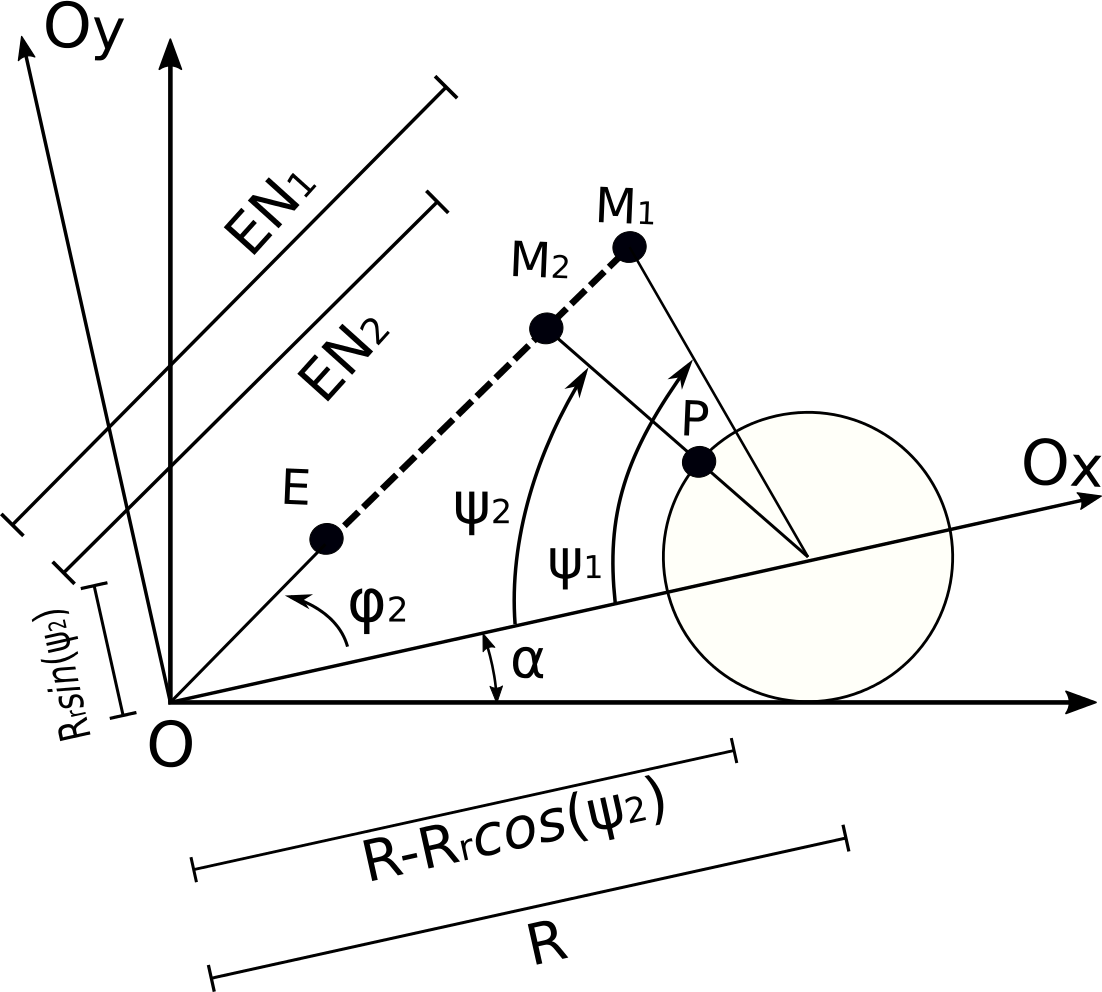
\includegraphics[width=0.50\linewidth]{fig/two_stage_angles}
   \caption{The angles for the second stage of the two-stage cycloid. The common normal through the contact point intersects at M\textsubscript{2} creating ange \textpsi\textsubscript{2}, but the actual instant center is dictated by the first stage at \textit{M\textsubscript{1}} defined by angle \textphi\textsubscript{1}.}
   \label{fig:two_stage_angles}
\end{figure}


In the single-stage design, the relative velocity of the two links along the common normal denoted as \texWtit{S} in Fig. \ref{fig:kennedy_sliding} is zero because the housing rollers are fixed in space. This holds true for the first stage of the two-stage concept, allowing calculation of their relative velocities using the same set of equations (\ref{eq:single_slide_offset} - \ref{eq:single_slide_vel}) However, in the second stage of the system, the housing rolers are moving in space, so there is some motion along S for the point P located on the second stage cycloid plate and second stage housing rollers. Figure \ref{fig:dual_relative_motion} shows these relative velocities for the second stage system. \textit{S} is the motion along the common normal for the point P on both links, \textit{M} is the motion of P on link 1 (the second stage cycloid plate) and \textit{L} is the motion of P on link 2 (the output housing rollers). 


\begin{figure}[h]
	\centering
	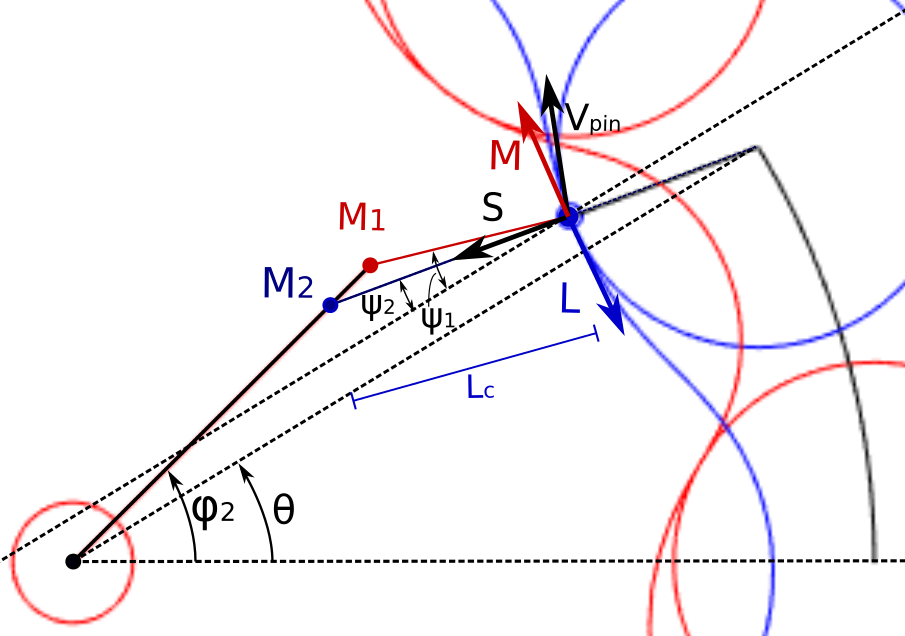
\includegraphics[width=0.50\linewidth]{fig/two_stage_vel_angles}
   \caption{Unlike the calculations for the relative velocities of the first stage of the cycloid, the second stage has output motion along the common normal, \textit{S}. The velocity of point P from the output velocity of the second stage, \textit{V\textsubscript(pin}} can be broken down into the \textit{S\textsubscript{pin}} and \textit{M}. The relative motion associated with the cycloid plate can be determined as \textit{S\textsubscript{plate}} and \texit{L}.}
   \label{fig:dual_relative_motion}
\end{figure}

First, \textit{S} and \textit{M} can be calculated for the motion of the output pins. The velocity of the output pins is the velocity of point P induced by the rotation of the output. A simplified drawing of this relationship is shown in Fig \ref{fig:dual_relative_motion}. This velocity \textit{V\textsubscript{o}} can be defined using the output angular velocity \textomega\textsubscript{o} and the length from the center to point P, \textit{L\textsubsript{op}} where \textpsi\textsubscript{2} is the angle used to calculate the profile of the second stage cycloid plate. An angular offset, \textit{offset\textsubscript{j}}, can be applied for each pin around the ring. 

\begin{equation}\label{eq:offset2}
offset_j = j \frac{2\pi}{N_2}
\end{equation}
\begin{equation}\label{eq:psi2}
\psi_2 = \taninv{\frac{E N_2 \sin(\phi_2-\alpha-offset_j)}{R-E N_2\cos(\phi_2-\alpha-offset_j)}}
\end{equation}
\begin{equation} \label{eq:l_op}
L_{op} = \sqrt{(R-R_r\cos\psi_2)^2 + (R_r\sin\psi_2)^2}
\end{equation}
\begin{equation}
\gamma = \taninv{\frac{R_r\sin\psi_2}{R-R_r\cos\psi_2}}
\end{equation}
\begin{equation}
V_{pin} = \frac{\omega_2}{Q} L_{op}
\end{equation}
\begin{equation} \label{eq:s_pin}
S_{pin} = \frac{\omega_2}{Q} L_{op} \cos(\frac{\pi}{2}-(\psi+\gamma))
\end{equation}
\begin{equation}
V_{1} = M = \frac{\omega_2}{Q} L_{op} \sin(\frac{\pi}{2}-(\psi+\gamma))
\end{equation}


Next, the velocity along the common normal, \textit{S} and the tangential velocity \textit{L} of point \textit{P} on the cycloid plate can be determined. If the calculations are correct, the velocity \textit{S} for both the pin, \textit{S\textsubscript{pin}} and \texit{S\textsubscript{plate}} are equal as they must move together to maintain contact. Figure \ref{fig:dual_relavite_motion} shows the geometric values needed to calculate these relative velocities. The angle difference between the angle used to calculate the cycloid profile \textpsi\textsubscript{2} and the actual angle of between the output roller center and the instant center caused by the first stage motion, \textpsi\textsubscript{1}, generate the motion along \textit{S} and \textit{L}. 

\begin{equation}\label{eq:psi_1}
\psi_1 = \taninv{\frac{E N_1 \sin(\phi_2-\alpha-offset_j) - R_r\sin\psi_2}
{R-R_r\cos\psi_2 - E N_1\cos(\phi_2-\alpha-offset_j)}}
\end{equation}
\begin{equation} \label{eq:psi_delta}
\psi_{\Delta} = \psi_2 - \psi_1
\end{equation}
\begin{equation}\label{eq:L_c}
L_{c} = \sqrt{\left[E N_1 \sin(\phi_2-\alpha-offset_j) - R_r\sin\psi_2\right]^2 + 
\left[R-R_r\cos\psi_2 - E N_1 \cos(\phi_2-\alpha-offset_j)\right]^2}
\end{equation}
\begin{equation}\label{eq:s_plate}
S_{plate} = \frac{\omega_2}{1-N_1} L_c \sin\psi_{\Delta}
\end{equation}
\begin{equation}\label{eq:L}
L = \frac{\omega_2}{1-N_1} L_c \cos\psi_{\Delta}
\end{equation}

It can be verified that through the motion, \texti{S\textsubscript{pin}} and \texit{S\textsubscript{plate}} are equal, showing that the relative motion of the point P along the common normal is in fact equal for both links, giving credence to the calculation method. Therefore, the relative velocity between the cycloid plate and the output pin can be caluclated as the difference betwen \textit{M} and \textit{L}.

\begin{equation}
V_{2} = M - L
\end{equation}

With these equations, the relative linear sliding velocity of the cycloid plate and pins for both the first stage and second stage plates can be analyzed throughout the motion. These velocity results can be combined with the force results to yield the predicted losses due to this interaction in the same way as the single-stage.

\begin{equation} \label{eq:dual_power_loss_1}
P_{L1} = \sum_{i=1}^{N_{1c}}\mu F_{1i} V_1
\end{equation}
\begin{equation} \label{eq:dual_power_loss_2}
P_{L2} = \sum_{j=1}^{N_{2c}}\mu F_2j V_2
\end{equation}


\section{Simulation and Test Results} \label{ch:dual:test_results}
% Go over the simulation results, loads in different conditions etc.
% - show the losses as a function of torque and velocity 
% - look at losses for different ratios of R/Rr 
% - show the predicted losses versus the actual losses of the designed cycloid. 

Using the equations laid out in Section \ref{ch:dual:equations}, the force and velocity on each lobe of a two-stage cycloidal drive can be calculated for a given arrangement. Using the NASA designed cycloid as a basis for comparison, studies were run to develop the relationship between positive and negative ratio, number of pins, and coefficient of friction to develop an understanding of the optimizations available in the design as well as compare to the ground truth of the NASA actuator. 

\subsection{Two-Stage Force and Velocity}\label{ch:dual:test_results:force_vel}
% Talk through the force and velocity on each pin. Show the graphs of the motion through space of the system. Probably can keep this short? 

The forces and velocities were calculated for the two-stage cycloid using the values set out in Table \ref{table:two_stage_design_params}. An example analysis is displayed in Fig \ref{fig:two_stage_forces}. For all presented analysis, a usage scenario of 0.25rad/s output RPM and 20Nm output torque was used as a basis for comparison. Therefore, for the NASA design, an input of 0.0309Nm and an input speed of 81 rad/s which, given a perfectly efficient system, would yield the desired outputs. 

\begin{figure}[h]
   \centering
   \begin{tabular}{cccc}
	   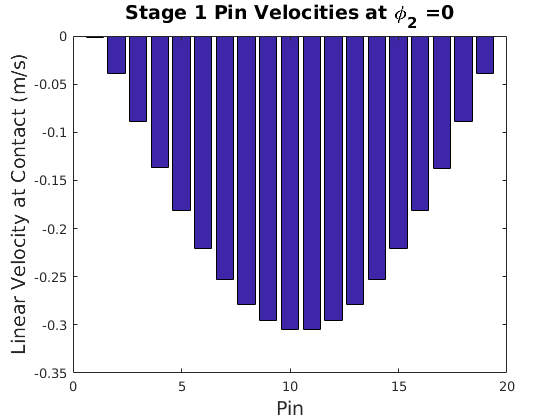
\includegraphics[width=0.23\textwidth]{fig/double_1_vel_0} &
	   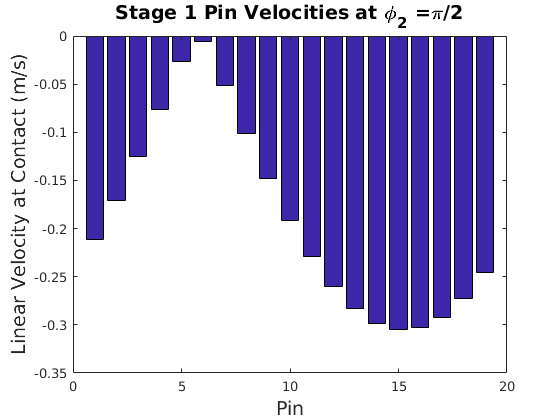
\includegraphics[width=0.23\textwidth]{fig/double_1_vel_pi_2} &
	   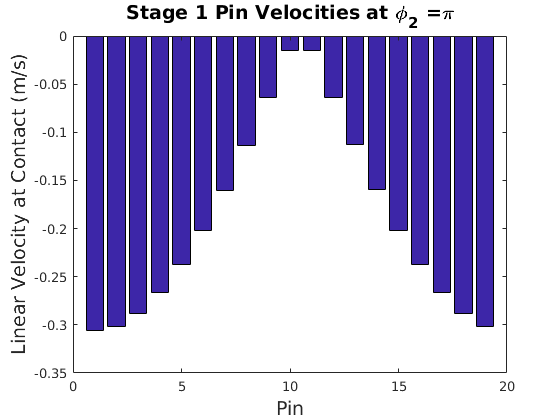
\includegraphics[width=0.23\textwidth]{fig/double_1_vel_pi} &
	   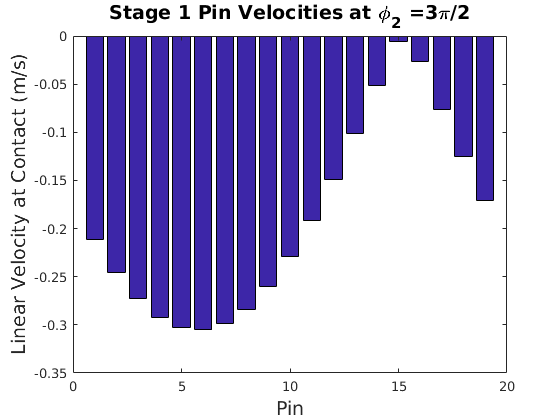
\includegraphics[width=0.23\textwidth]{fig/double_1_vel_3pi_2} \\
	   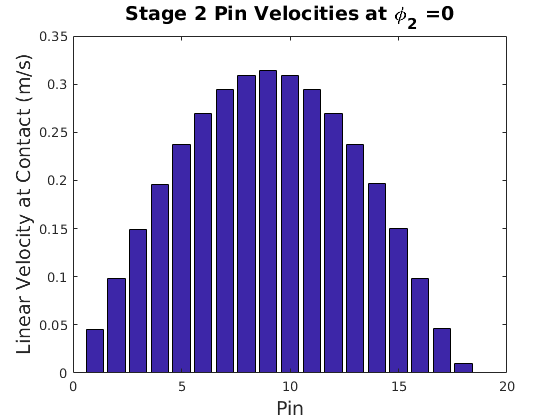
\includegraphics[width=0.23\textwidth]{fig/double_2_vel_0} &
	   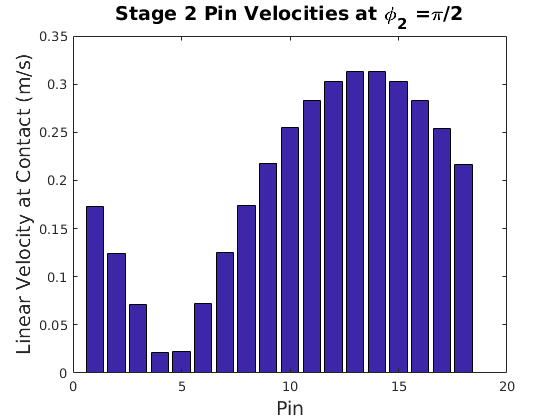
\includegraphics[width=0.23\textwidth]{fig/double_2_vel_pi_2} &
	   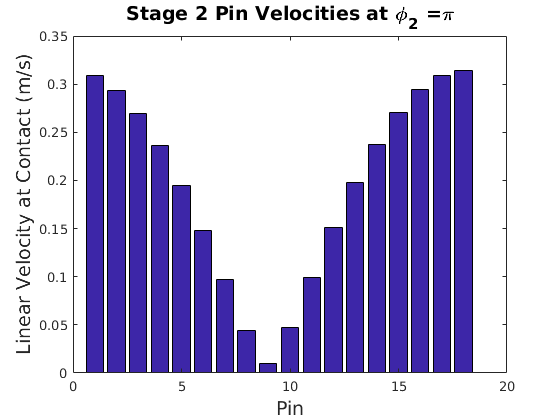
\includegraphics[width=0.23\textwidth]{fig/double_2_vel_pi} &
	   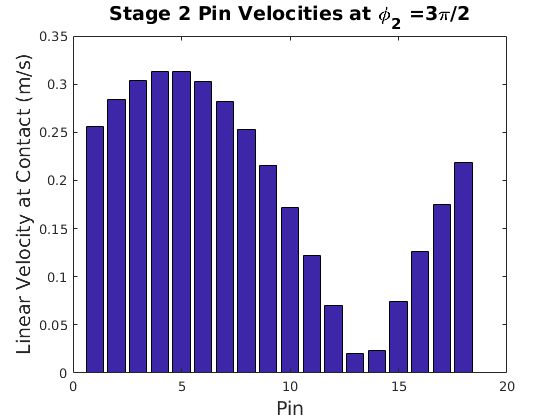
\includegraphics[width=0.23\textwidth]{fig/double_2_vel_3pi_2} \\
	   \\
	   \hline
	   \\
	   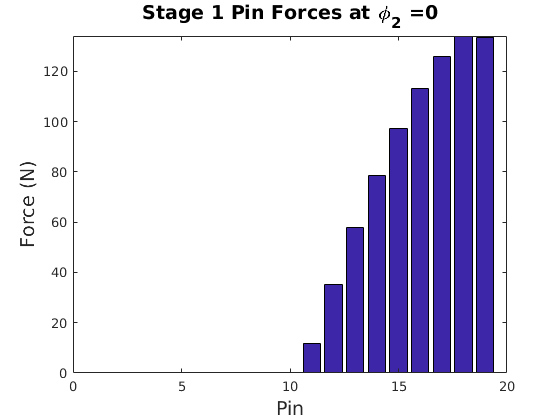
\includegraphics[width=0.23\textwidth]{fig/double_1_forces_0} &
	   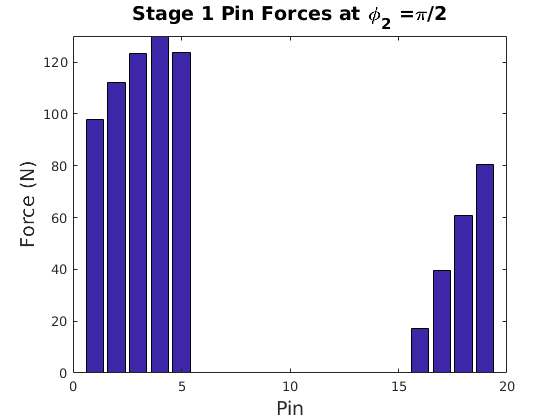
\includegraphics[width=0.23\textwidth]{fig/double_1_forces_pi_2} &
	   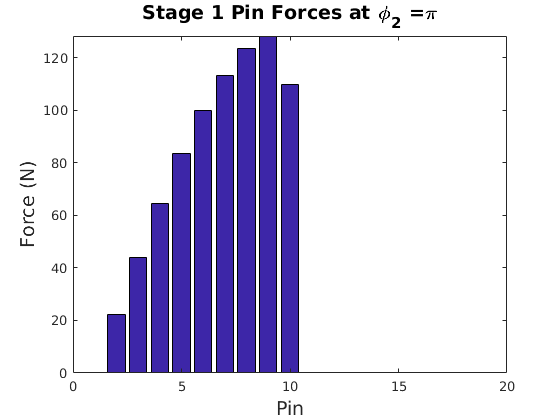
\includegraphics[width=0.23\textwidth]{fig/double_1_forces_pi} &
	   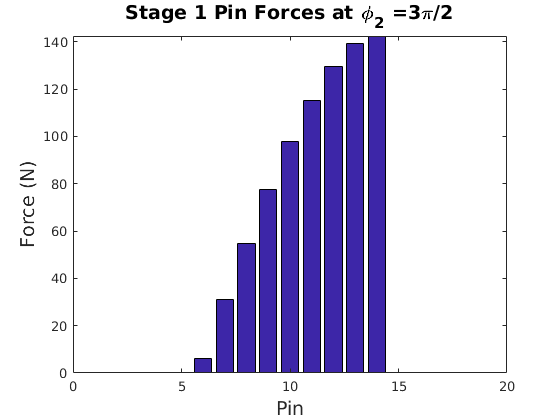
\includegraphics[width=0.23\textwidth]{fig/double_1_forces_3pi_2} \\
	   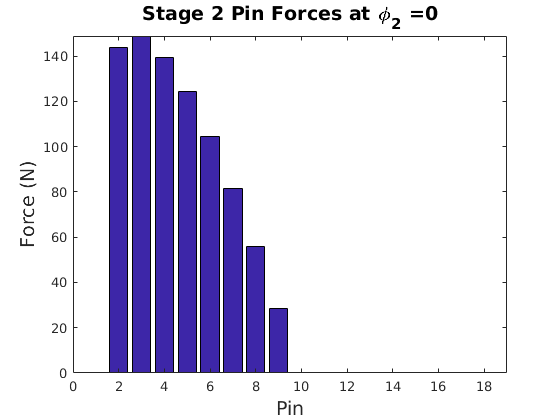
\includegraphics[width=0.23\textwidth]{fig/double_2_forces_0} &
	   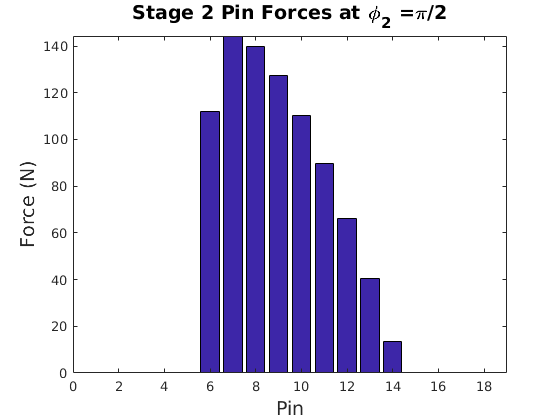
\includegraphics[width=0.23\textwidth]{fig/double_2_forces_pi_2} &
	   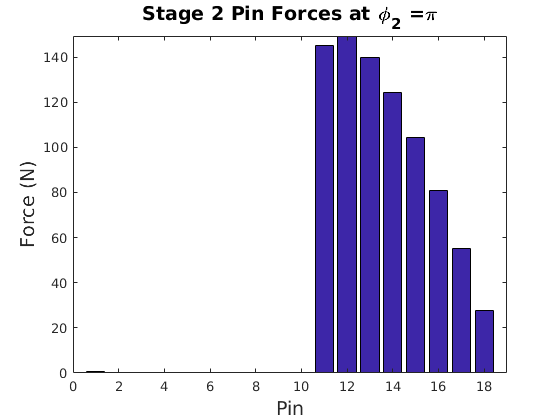
\includegraphics[width=0.23\textwidth]{fig/double_2_forces_pi} &
	   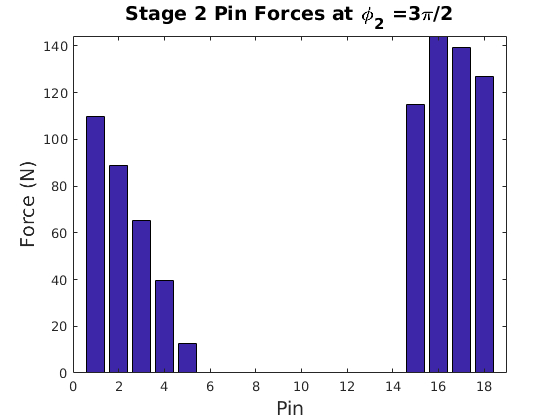
\includegraphics[width=0.23\textwidth]{fig/double_2_forces_3pi_2} \\
	   \\
	   \hline
	   \\
	   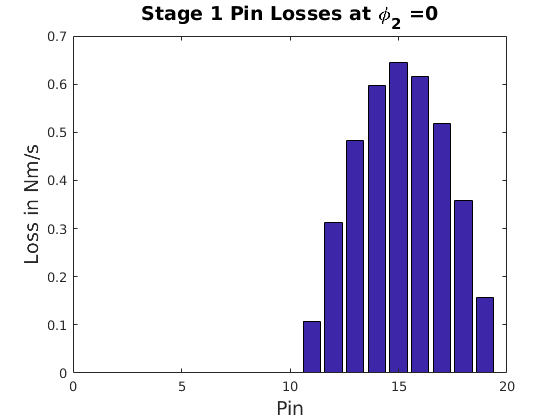
\includegraphics[width=0.23\textwidth]{fig/double_1_losses_0} &
	   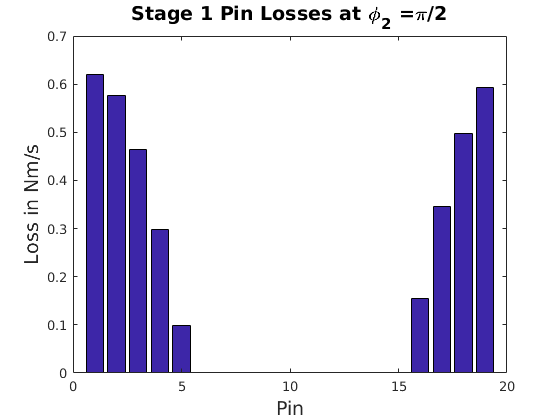
\includegraphics[width=0.23\textwidth]{fig/double_1_losses_pi_2} &
	   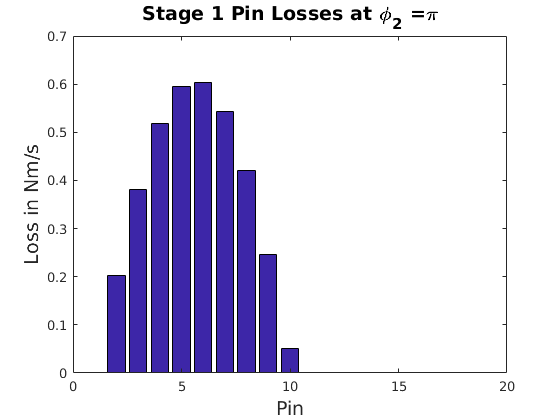
\includegraphics[width=0.23\textwidth]{fig/double_1_losses_pi} &
	   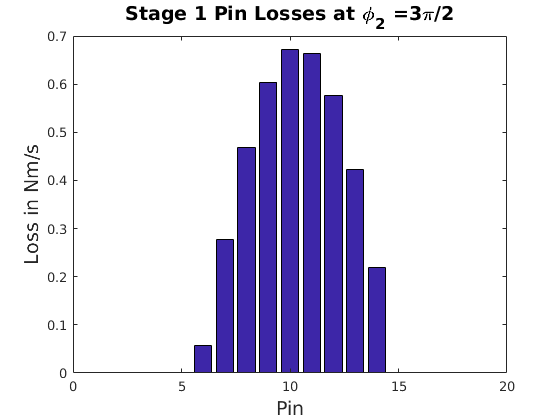
\includegraphics[width=0.23\textwidth]{fig/double_1_losses_3pi_2} \\
	   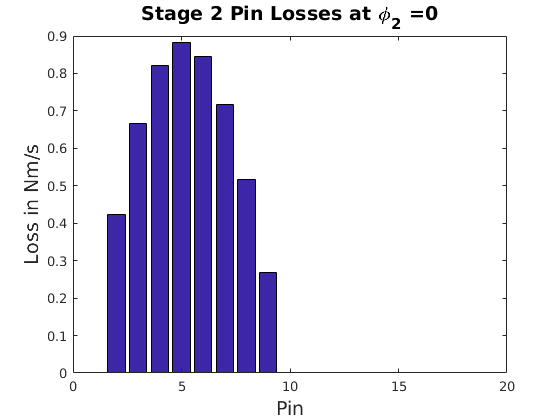
\includegraphics[width=0.23\textwidth]{fig/double_2_losses_0} &
	   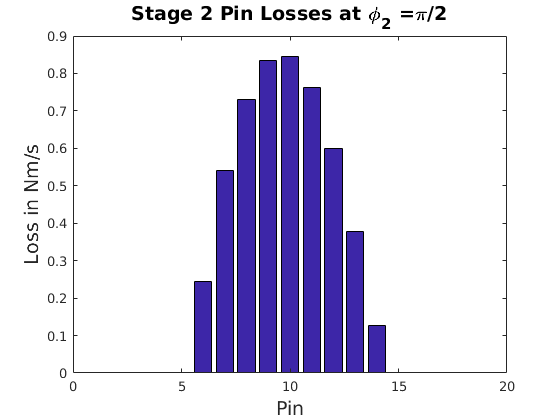
\includegraphics[width=0.23\textwidth]{fig/double_2_losses_pi_2} &
	   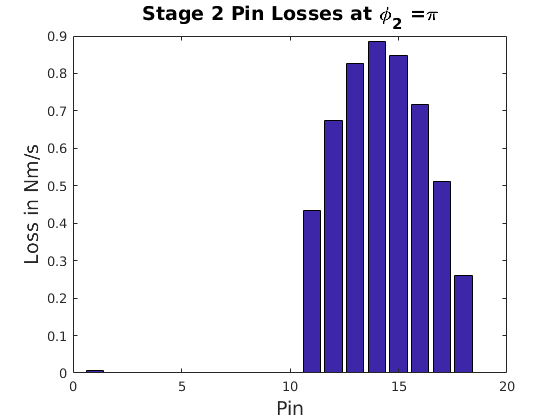
\includegraphics[width=0.23\textwidth]{fig/double_2_losses_pi} &
	   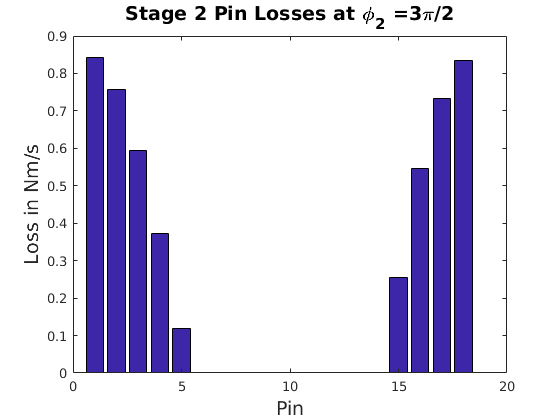
\includegraphics[width=0.25\textwidth]{fig/double_2_losses_3pi_2} \\
   \end{tabular}
   \caption{Full set of velocities, forces, and losses through a single input rotation of a two-stage cycloid system with a positive 324:1 ratio.}
   \label{fig:two_stage_forces}
\end{figure}

\begin{figure}[h]
   \centering
   \begin{tabular}{cccc}
	   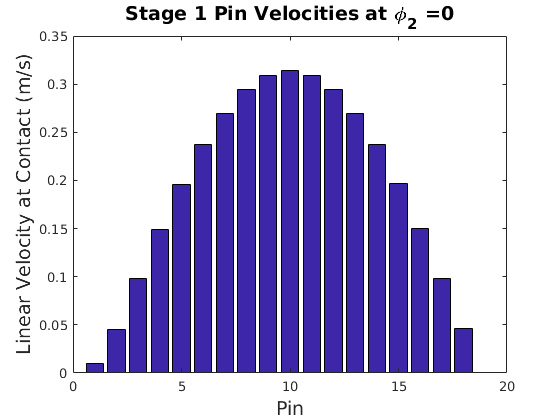
\includegraphics[width=0.23\textwidth]{fig/double_1_neg_vel_0} &
	   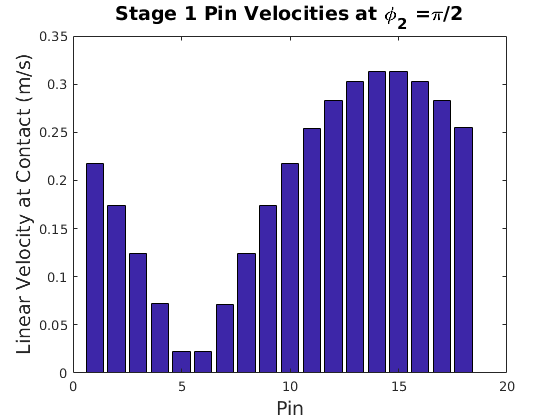
\includegraphics[width=0.23\textwidth]{fig/double_1_neg_vel_pi_2} &
	   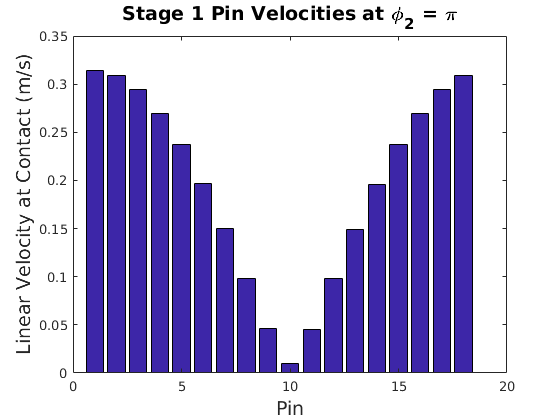
\includegraphics[width=0.23\textwidth]{fig/double_1_neg_vel_pi} &
	   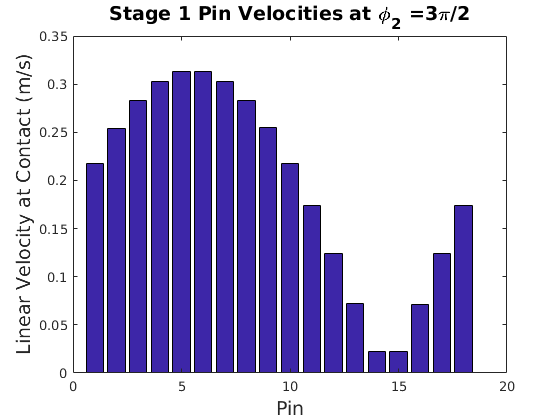
\includegraphics[width=0.23\textwidth]{fig/double_1_neg_vel_3pi_2} \\
	   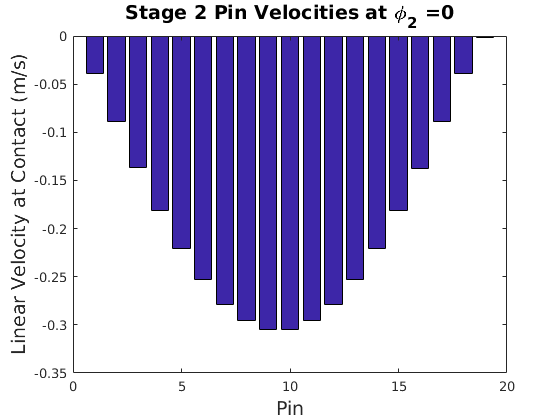
\includegraphics[width=0.23\textwidth]{fig/double_2_neg_vel_0} &
	   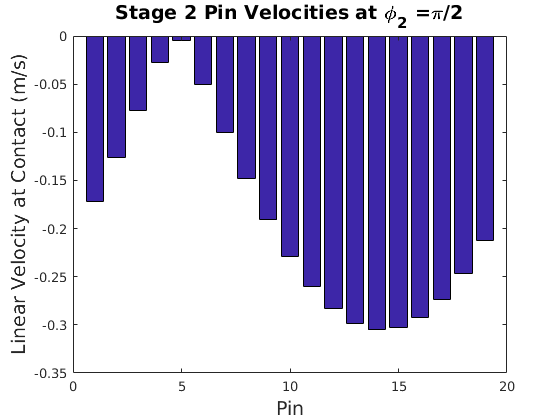
\includegraphics[width=0.23\textwidth]{fig/double_2_neg_vel_pi_2} &
	   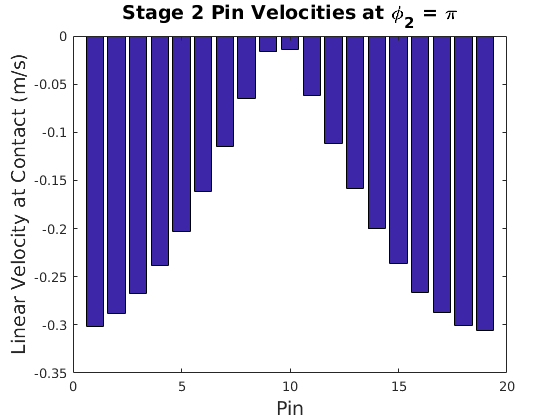
\includegraphics[width=0.23\textwidth]{fig/double_2_neg_vel_pi} &
	   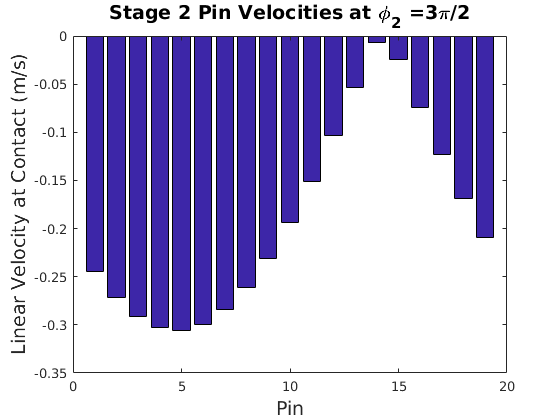
\includegraphics[width=0.23\textwidth]{fig/double_2_neg_vel_3pi_2} \\
	   \\
	   \hline
	   \\
	   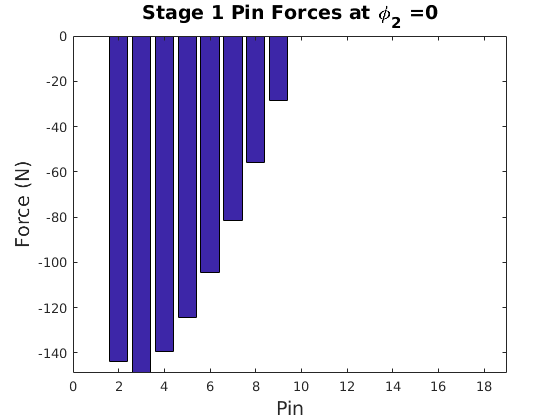
\includegraphics[width=0.23\textwidth]{fig/double_1_neg_forces_0} &
	   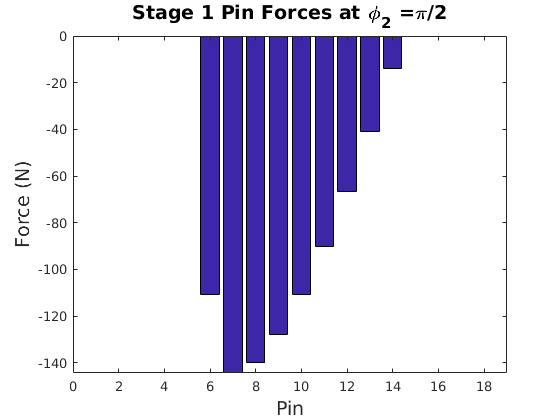
\includegraphics[width=0.23\textwidth]{fig/double_1_neg_forces_pi_2} &
	   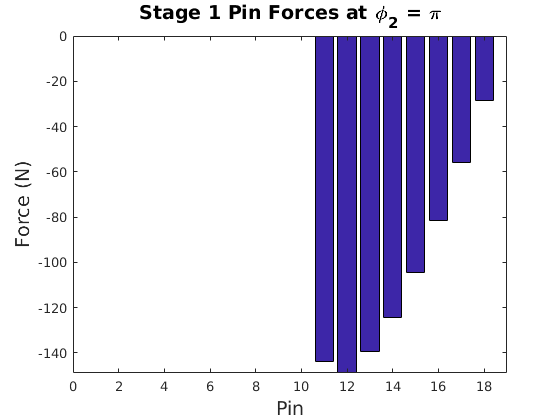
\includegraphics[width=0.23\textwidth]{fig/double_1_neg_forces_pi} &
	   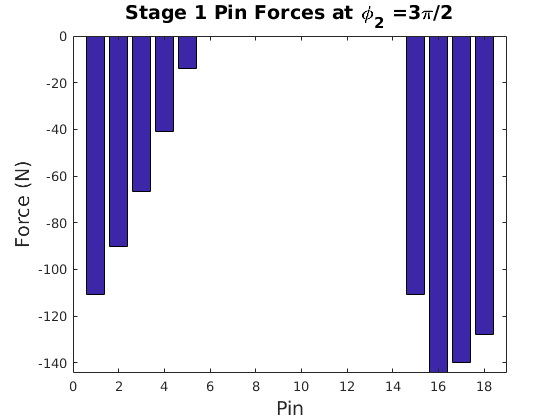
\includegraphics[width=0.23\textwidth]{fig/double_1_neg_forces_3pi_2} \\
	   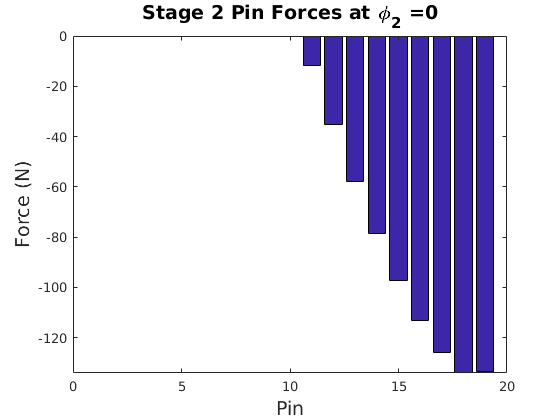
\includegraphics[width=0.23\textwidth]{fig/double_2_neg_forces_0} &
	   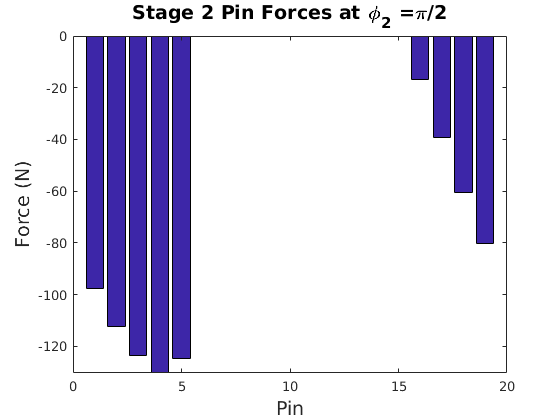
\includegraphics[width=0.23\textwidth]{fig/double_2_neg_forces_pi_2} &
	   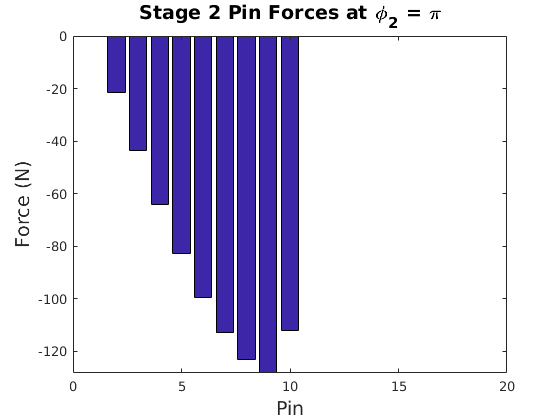
\includegraphics[width=0.23\textwidth]{fig/double_2_neg_forces_pi} &
	   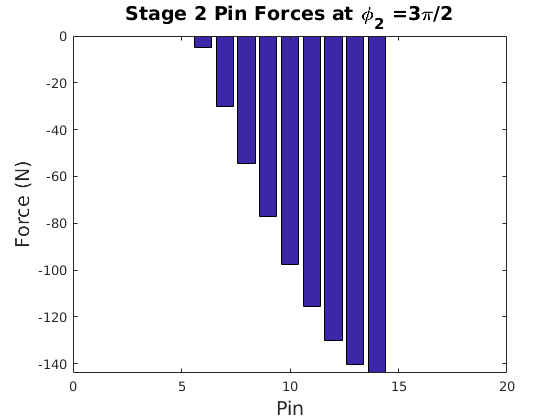
\includegraphics[width=0.23\textwidth]{fig/double_2_neg_forces_3pi_2} \\
	   \\
	   \hline
	   \\
	   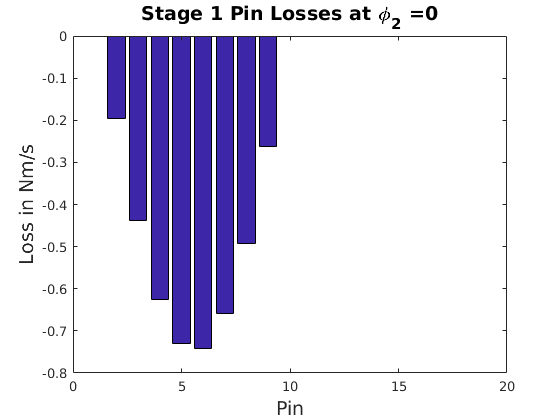
\includegraphics[width=0.23\textwidth]{fig/double_1_neg_losses_0} &
	   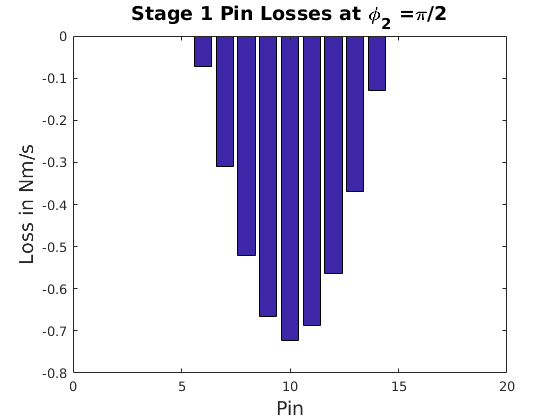
\includegraphics[width=0.23\textwidth]{fig/double_1_neg_losses_pi_2} &
	   \includegraphics[width=0.23\textwidth]{fig/double_1_neg_losses_pi} &
	   \includegraphics[width=0.23\textwidth]{fig/double_1_neg_losses_3pi_2} \\
	   \includegraphics[width=0.23\textwidth]{fig/double_2_neg_losses_0} &
	   \includegraphics[width=0.23\textwidth]{fig/double_2_neg_losses_pi_2} &
	   \includegraphics[width=0.23\textwidth]{fig/double_2_neg_losses_pi} &
	   \includegraphics[width=0.25\textwidth]{fig/double_2_neg_losses_3pi_2} \\
   \end{tabular}
   \caption{Full set of velocities, forces, and losses through a single input rotation of a two-stage cycloid system with a negative 323:1 ratio.}
   \label{fig:two_stage_forces}
\end{figure}

This can be contrasted with the similar design but utilizing a negative ratio by inverting which cycloid plate has more pins. If the first stage has more pins, the ratio will be positive, if the second stage has more pins, it will be negative. So while the parameters in Table \ref{table:two_stage_design_params} results in a ratio of 324:1, the reverse arrangement in Table \ref{table:two_stage_invert_design_params} results in a ratio of -323:1. The same input motion simulated for the first arrangement is applied to the reverse arrangement and shown in Figure \ref{fig:two_stage_forces_rev}.

\subsection{Two-Stage Lobe to Pin Losses} \label{ch:dual:test_results:losses}
% Show the plots of the losses for the different combinations of things. Show 324 to -323, 324 - 151 - whatever, 324 to 334 

An analysis of the predicted losses for a two-stage cycloid was conducted using the forces and velocities laid out in Section \ref{ch:dual:test_results:force_vel} using equations \ref{eq:dual_power_loss_1} and \ref{eq:dual_power_loss_2} for a range of coefficients of friction. This result can be seen in Fig \ref{fig:two_stage_as_designed}.

\begin{figure}[h]
	\centering
	\includegraphics[width=0.75\linewidth]{fig/two_stage_as_designed}
   \caption{The predicted efficiency of the NASA two-stage cycloid for a range of coefficients of friction}
   \label{fig:two_stage_as_designed}
\end{figure}

This efficiency analysis can be contrasted against the tested values of the NASA designed two-stage cycloid system. The constructed actuator was run through a break in period of approximately 10 hours. During this time, the efficiency of the system was not observed to change appreciably. A test cycle, outlined in Table \ref{table:two_stage_test_cycle} was run over the course of TODO hours. The testing was run using the same setup as outlined in Section \ref{ch:single:test_setup}. The two stage was mounted in the same location as the single-stage and run with the same control equipment. The results of this cycling can be seen in Fig \ref{fig:two_stage_results}.

\begin{figure}[h]
	\centering
	\includegraphics[width=0.75\linewidth]{fig/two_stage_eff}
   \caption{The efficiency over time of the NASA designed two-stage cycloid system. Each line corresponds to one of the test conditions that varied over time, outlined in Table \ref{table:two_stage_test_cycle}.}
   \label{fig:two_stage_eff}
\end{figure}

Only a modest drive cycle was run on the actuator, as it's efficiencies were much lower than anticipated, therefore, the current load on the system was too high to achieve higher torques due to both over-current and over-temperature conditions. This result is what lead to the additional analysis to study the predicted losses of the system with the pin-in-housing design for a two-stage. The peak efficiency observed for the cycloid was 36\%. This suggests that the coefficient of friction achieved between the rollers and housing was approximately 0.03 using Fig \ref{fig:two_stage_as_designed}. This result will be discussed in detail in Section \ref{ch:dual:discussion:actual}.


\section{Discussion} \label{ch:dual:discussion}
% Two-stages aren't awesome because you have such a multiplication of force, and the loss scales more sharply with force (not to mention the huge multiplcation of velocity too for that matter that scales by a different factor) and that causes pretty inefficient designs for this compact style. They should be built with rolling elements based on this analysis, and no one has said that yet, so boom bitches. 
% Additionally, if trying to minimize losses, you should build it negative, and you get reduced losses for more pins. 

This force and velocity analysis demonstrates an number of new and interesting revelations about the functionality of two-stage cycloids. First, the comparison between the calculated efficiencies and the achieved efficiency of the as built actuator gives indications to design of these systems. Next, the arrangement of the pins for a positive or negative ratio influences the losses in the system, the number of pins in the system influences losses, and the overall ratio to yield the same output velocity and force also influences losses. These will be discussed in detail in this section. For each comparative analysis, the system was setup to yield an output torque of 20Nm, and an output velocity of 0.25rad/s, in line with the tested NASA reducer.

\subsection{Analysis of Pin-in-Housing Two-Stage Cycloid} \label{ch:dual:discussion:actual}

An important result stems from the comparison of the actual performance of a two-stage cycloid using pins in the housing to the theoretical calculations. For the size of the ratio desired for the design, the peak efficiency quickly falls off as the coefficient of friction increases. Coefficients of friction for lubricated steel to steel can be found from many on-line sources, and generally range from 0.03 - 0.15. Given this, if pins resting in the housing are used as they are in a compact single-stage design, with the lowest reasonable coefficient of friction of 0.03, the efficiency loss associated with just this interaction brings the peak efficiency to 36\%, not including any other losses from bearing elements. The tested cycloid efficiency was in this same range, so if the built cycloid may have been achieving a nearly optimal coefficient of friction between the pins and the housing. However, even with this nearly optimal coefficient of friction, the losses are still substantial for this design. 


A generally accepted ``efficient'' system (\textless90\%) is not achieved until the coefficient of friction of \textless0.002 which is only achieved with roller bearings. Therefore, if a designer needs an incredibly large ratio, such as the one designed and tested, rolling elements may need to be employed at all lobe to pin interfaces to allow higher efficiencies to be achieved. This will potentially drastically increase the mass and size of a two-stage system from those proposed in the literature and the one designed. However, the trade between this larger, heavier design may still lean in favor of a two-stage cycloid versus other series reductions to achieve a similar result. This analysis is left to future work. 

\subsection{Positive and Negative Ratio Arrangement}\label{ch:dual:discussion:pos_neg}

The first comparison to analyze is the choice of positive or negative arrangement. The most apparent difference between the positive and negative arrangements is the loads are flipped as the input goes around. That is, in Fig \ref{fig:two_stage_forces}, the loads are on pins 1-TODO on stage one and TODO-TODO on stage 2, while in Fig \ref{fig:two_stage_forces_rev} this is flipped, so stage 1 has loads on pins TODO-TODo and stage 2 has loads on pins TODO-TODO. Additionally, in the positive arrangement, the load is slightly lower per pin on the first stage because there are more pins and lobes and higher on the second stage. This is reversed in the negative arrangement. 

\begin{figure}[h]
	\centering
	\includegraphics[width=0.75\linewidth]{fig/two_stage_pos_neg}
   \caption{A comparison of efficiencies over friction coefficients for the positive and negative ratios using the design parameters laid out in Table \ref{table:two_stage_design_params} and Table \ref{table:two_stage_invert_design_params}}
   \label{fig:two_stage_pos_neg}
\end{figure}

While it would appear that these loads are equally flipped, and would therefore cancel out, the coupling of these loads and the relative velocities of the pins to cycloid plates plays into the predicted losses of the system, in which loss is proportional to both force and velocity. Because there is more relative motion between the cycloid plate and the pins in the second stage plate, as evident in both Fig \ref{fig:two_stage_forces} and Fig \ref{two_stage_forces_rev}, if the load is higher on the second stage plates due to this increased velocity condition, losses will increase. This relationship causes the disparity in losses for positive and negative ratios that is demonstrated in Fig \ref{fig:two_stage_pos_neg}, where the negative ratio has a lower loss per  unit of coefficient of friction. This result suggests that, whenever possible, a designer should opt for a negative ratio arrangement to decrease the losses of the actuator. 



\subsection{Number of Lobes Effect on Efficiency}\label{ch:dual:discussion:num_lobes}

The second interesting comparison that can be done using the predicted efficiencies is the effect of the number of lobes and pins on the efficiency. The more efficient negative ratio of -323:1 was compared to as theoretical design of a -333.3:1 ratio using over twice as many pins. The design parameters for this higher pin number design were taken from the single-stage design and applied to a two stage design. These design parameters are listed in Tab;e \ref{table:two_stage_high_pins}. 

\begin{table}[h]
  \vskip0.2cm
  \caption{Design parameters for a similar reduction with nearly 3x the number of pins}
  \label{table:two_stage_high_pins}
  \begin{center}
    \vskip-0.2cm
	\begin{tabular}{|c|c|c|}
		\hline
		Variable & Symbol & Value\\
		\hline
		Stage 1 Housing Rollers & \textit{N\textsubscript{1}} & 51\\
		\hline
		Stage 1 Lobes & N/A & 50\\
		\hline
		Stage 2 Housing Rollers & \textit{N\textsubscript{2}} & 60\\
		\hline
		Stage 2 Lobes & N/A & 59\\
		\hline
		Total Ratio & \textit{Q} & -333.3:1 \\
		\hline
		Roller Offset & \textit{R} & 50.8mm \\
		\hline
		Roller Diaeter & \textit{R\textsubscript{r}} & 1.588 mm\\
		\hline
	\end{tabular}
  \end{center}
\end{table}

\begin{figure}[h]
	\centering
	\includegraphics[width=0.75\linewidth]{fig/two_stage_more_pins}
   \caption{A comparison of the efficiencies over friction coefficient for two similar ratios, one using 18 stage 1 lobes and 19 stage 2 lobes, the second using 51 stage 1 lobes and 60 stage 2 lobes.}
   \label{fig:two_stage_more_pins}
\end{figure}

The theoretical efficiencies of these two systems can be seen in Fig \ref{fig:two_stage_more_pins}. This indicates that as the number of interacting pins increases, the efficiency increases. This results suggests that, where possible, a designer should use more, potentially smaller, pins in a design than few large pins to achieve more optimal efficiencies. 


\subsection{Effect of Ratio on Efficiency} \label{ch:dual:discussion:ratio}

\begin{figure}[h]
	\centering
	\includegraphics[width=0.75\linewidth]{fig/two_stage_lower_ratio}
   \caption{A comparison of the efficiencies over friction coefficient for a two dissimilar with torque and velocity inputs to achieve equal outputs. The first uses 18 stage 1 lobes and 19 stage 2 lobes, the second uses 17 stage 1 lobes and 19 stage 2 lobes}
   \label{fig:two_stage_lower_ratio}
\end{figure}


\begin{table}[h]
  \vskip0.2cm
  \caption{Design parameters for a similar design using one fewer first stage lobes, resulting in ~1/2 the ratio.}
  \label{table:two_stage_lower_ratio}
  \begin{center}
    \vskip-0.2cm
	\begin{tabular}{|c|c|c|}
		\hline
		Variable & Symbol & Value\\
		\hline
		Stage 1 Housing Rollers & \textit{N\textsubscript{1}} & 17\\
		\hline
		Stage 1 Lobes & N/A & 16\\
		\hline
		Stage 2 Housing Rollers & \textit{N\textsubscript{2}} & 19\\
		\hline
		Stage 2 Lobes & N/A & 18\\
		\hline
		Total Ratio & \textit{Q} & -152:1 \\
		\hline
		Roller Offset & \textit{R} & 38.1mm \\
		\hline
		Roller Diaeter & \textit{R\textsubscript{r}} & 3.97 mm\\
		\hline
	\end{tabular}
  \end{center}
\end{table}

The final interesting comparison that was made was the effect of ratio on the efficiency. A ratio of -323:1 was compared to a ratio of -152:1, using 1 fewer rollers and lobes on the first stage, laid out in Table \ref{table:two_stage_lower_ratio}. With the input torque and velocity scaling to achieve the same output, the predicated efficiencies are presented in Fig \ref{fig:two_stage_lower_ratio}. This result is intuitive to many designers, that a lower ratio results in a higher efficiency and should not come as a surprise. This is confirmed using this analysis. With this design, the cycloid itself would need to change very little to achieve this half ratio, as the loads carried by the rollers and lobes will only increase as a ratio of the total lobes of the first ratio to the total lobes of the second ratio because they all carry the output torque desired. The only major change in the design would be the motor used as the input that would need to double in potential torque output. This motor increase will likely lead to a gain in mass for a given design. Therefore, if optimal efficiency is more important than total mass, a lower reduction should be considered. 

